\documentclass[a4paper,12pt]{article}
\usepackage[utf8]{inputenc}
\usepackage[cm,empty]{fullpage}
\usepackage[T2A]{fontenc}
\usepackage[english, russian]{babel}
\usepackage{amssymb,amsmath,amsxtra,amsthm}
\usepackage{proof}
\usepackage[pdftex]{graphicx}
\usepackage{wrapfig}
\usepackage{skak}

\usepackage[left=2cm,right=2cm,
    top=1cm,bottom=1cm,bindingoffset=0cm]{geometry}

\renewcommand{\leq}{\leqslant}
\renewcommand{\geq}{\geqslant}


\newcommand{\iiff}{\Longleftrightarrow}
\renewcommand{\iff}{\Leftrightarrow}
\newcommand{\nothing}{\varnothing}


\newcommand{\NN}{\mathbb{N}}
\newcommand{\ZZ}{\mathbb{Z}}
\newcommand{\Q}{\mathbb{Q}}
\newcommand{\A}{\mathbb{A}}
\newcommand{\R}{\mathbb{R}}
\renewcommand{\C}{\mathbb{C}}

\renewcommand{\phi}{\varphi}
\newcommand{\eps}{\varepsilon}

\newcounter{z}


\newcommand{\zs}{\refstepcounter{z}\vskip 10pt\par\noindent
\fbox{\textbf{12.\arabic{z}}} }

\newcommand{\z}{\refstepcounter{z}\vskip 20pt\noindent
\fbox{\textbf{\arabic{z}}} }

\renewcommand{\date}{{\bf 27 января 2021}} %Дата занятия

\newcommand{\dif}
{
------------------------------------------------------------------------------------------------------------------------------------------------------
}

\newcommand{\HSEhat}{
\vspace*{-0pt}
\noindent
\setcounter{z}{0}
\vspace*{-10pt}
\begin{wrapfigure}[2]{l}{5pt}
\vspace*{-25pt}
\hspace*{-20pt}

\includegraphics[scale=0.18]{img/HSE_LOGO.png}
\end{wrapfigure}
\vspace{-20pt}


{\bf \phantom{\date}  \large \hfill Дискретная математика: \hfill \normalsize \date}

\vspace{5 pt}
{\bf \large \hfill  неориентированные графы.\hfill }

\vspace{15 pt}
\centerline{ \large  Домашнее задание.}



\vspace*{10pt}
\setcounter{z}{0}

}

\begin{document}

\HSEhat

Всюду ниже рассматриваются только графы {\bf без петель} и {\bf кратных ребер}.


\begin{center}
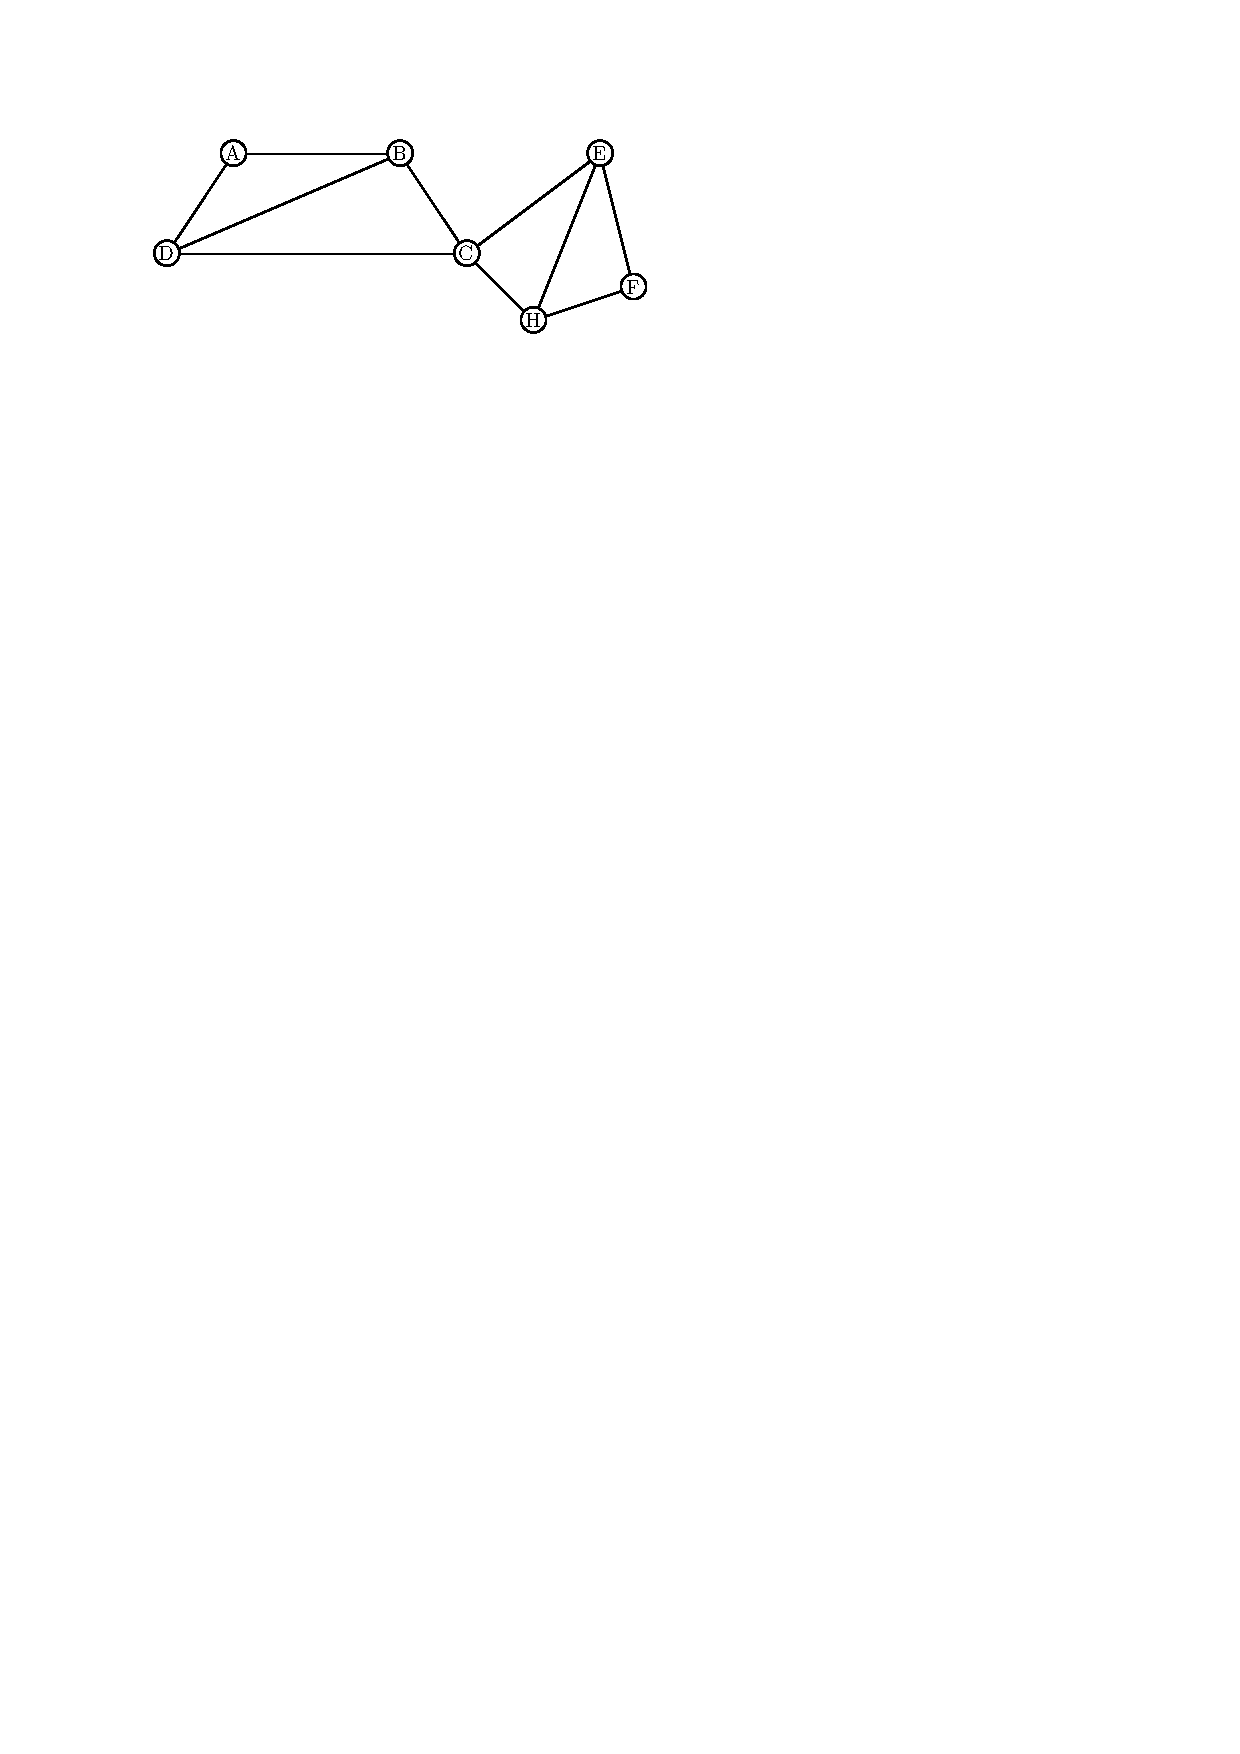
\includegraphics[scale=1]{img/graphHW.pdf}
\end{center}
\vspace{-15 pt}

\z Граф $G$ изображен на рисунке выше.

{\bf а)} Найдите максимальную длину простого цикла в графе $G$. Укажите
все различные простые циклы максимальной длины.

{\bf б)} Верно ли, что если в графе $G$ удалить любое ребро, то из любой его
вершины можно будет добраться до любой? При положительном ответе
приведите обоснование, при отрицательном --- укажите ребро, которое
можно удалить, и вершины, между которыми не будет пути.

{\bf в)} Какое минимальное количество рёбер необходимо удалить из графа $G$, чтобы он стал несвязным?


\z В государстве $100$ городов, и из каждого из них выходит $4$ дороги в другие города этого государства. Сколько всего дорог в государстве?

\z Можно ли нарисовать картинки на рисунке ниже, не отрывая карандаша от бумаги и проходя по каждой линии по одному разу?

Если можно, то покажите, как это сделать.

Если нельзя, то докажите, что это сделать невозможно.
\vspace{-40 pt}
\begin{center}
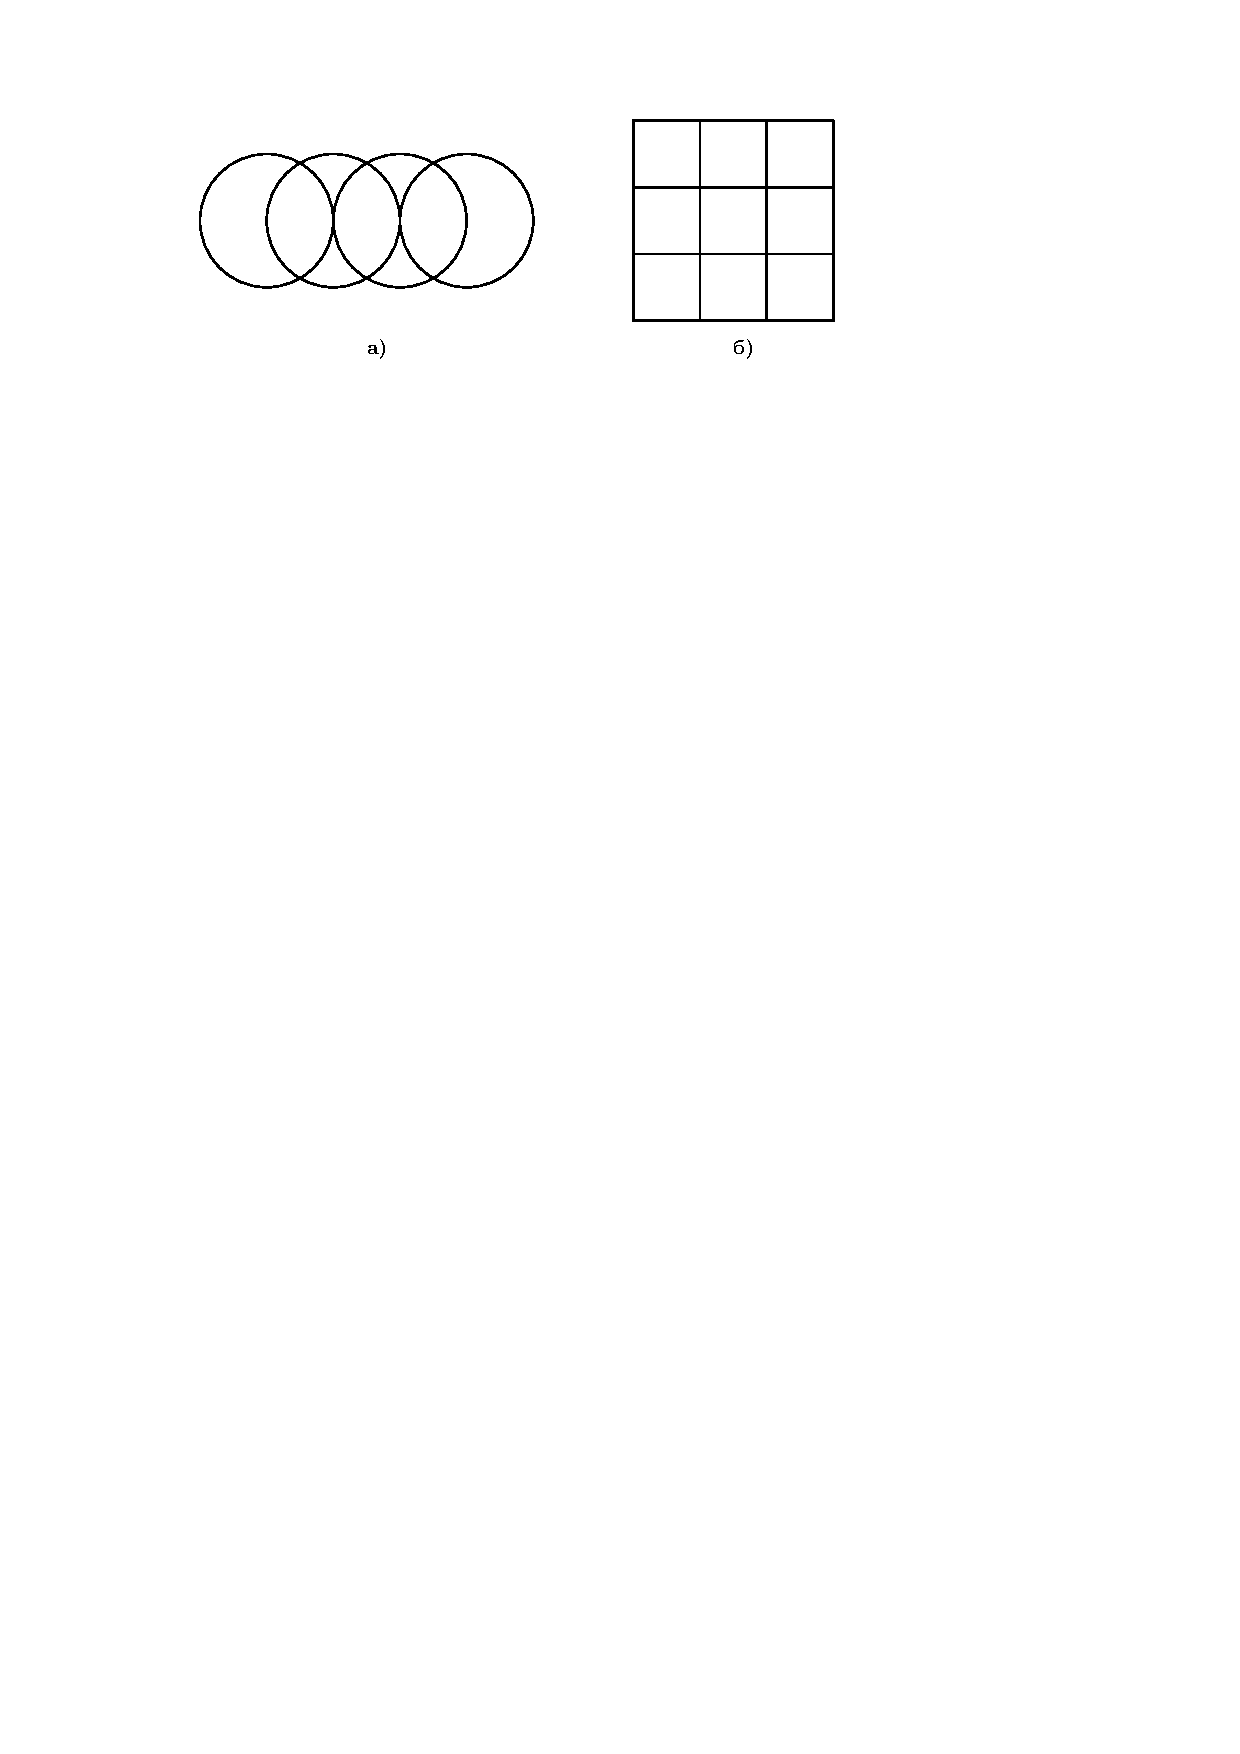
\includegraphics[scale=1]{img/graphHW2.pdf}
\end{center}
\vspace{-15 pt}

\z В дереве на $2020$ вершинах ровно три вершины имеют степень $1$.
Сколько вершин имеют степень $3$?

\newpage

\z У некоторого графа на $6$ вершинах ровно $11$ ребер. Докажите, что этот граф связен.



\z Можно ли за несколько ходов (по шахматным правилам и не выходя за пределы доски $3\times 3$) поставить коней так, чтобы из расположения на левой картинке получилось расположение коней на правой?

Если можно, то укажите последовательность шагов.

Если нельзя, то докажите, что это сделать невозможно.

\begin{center}
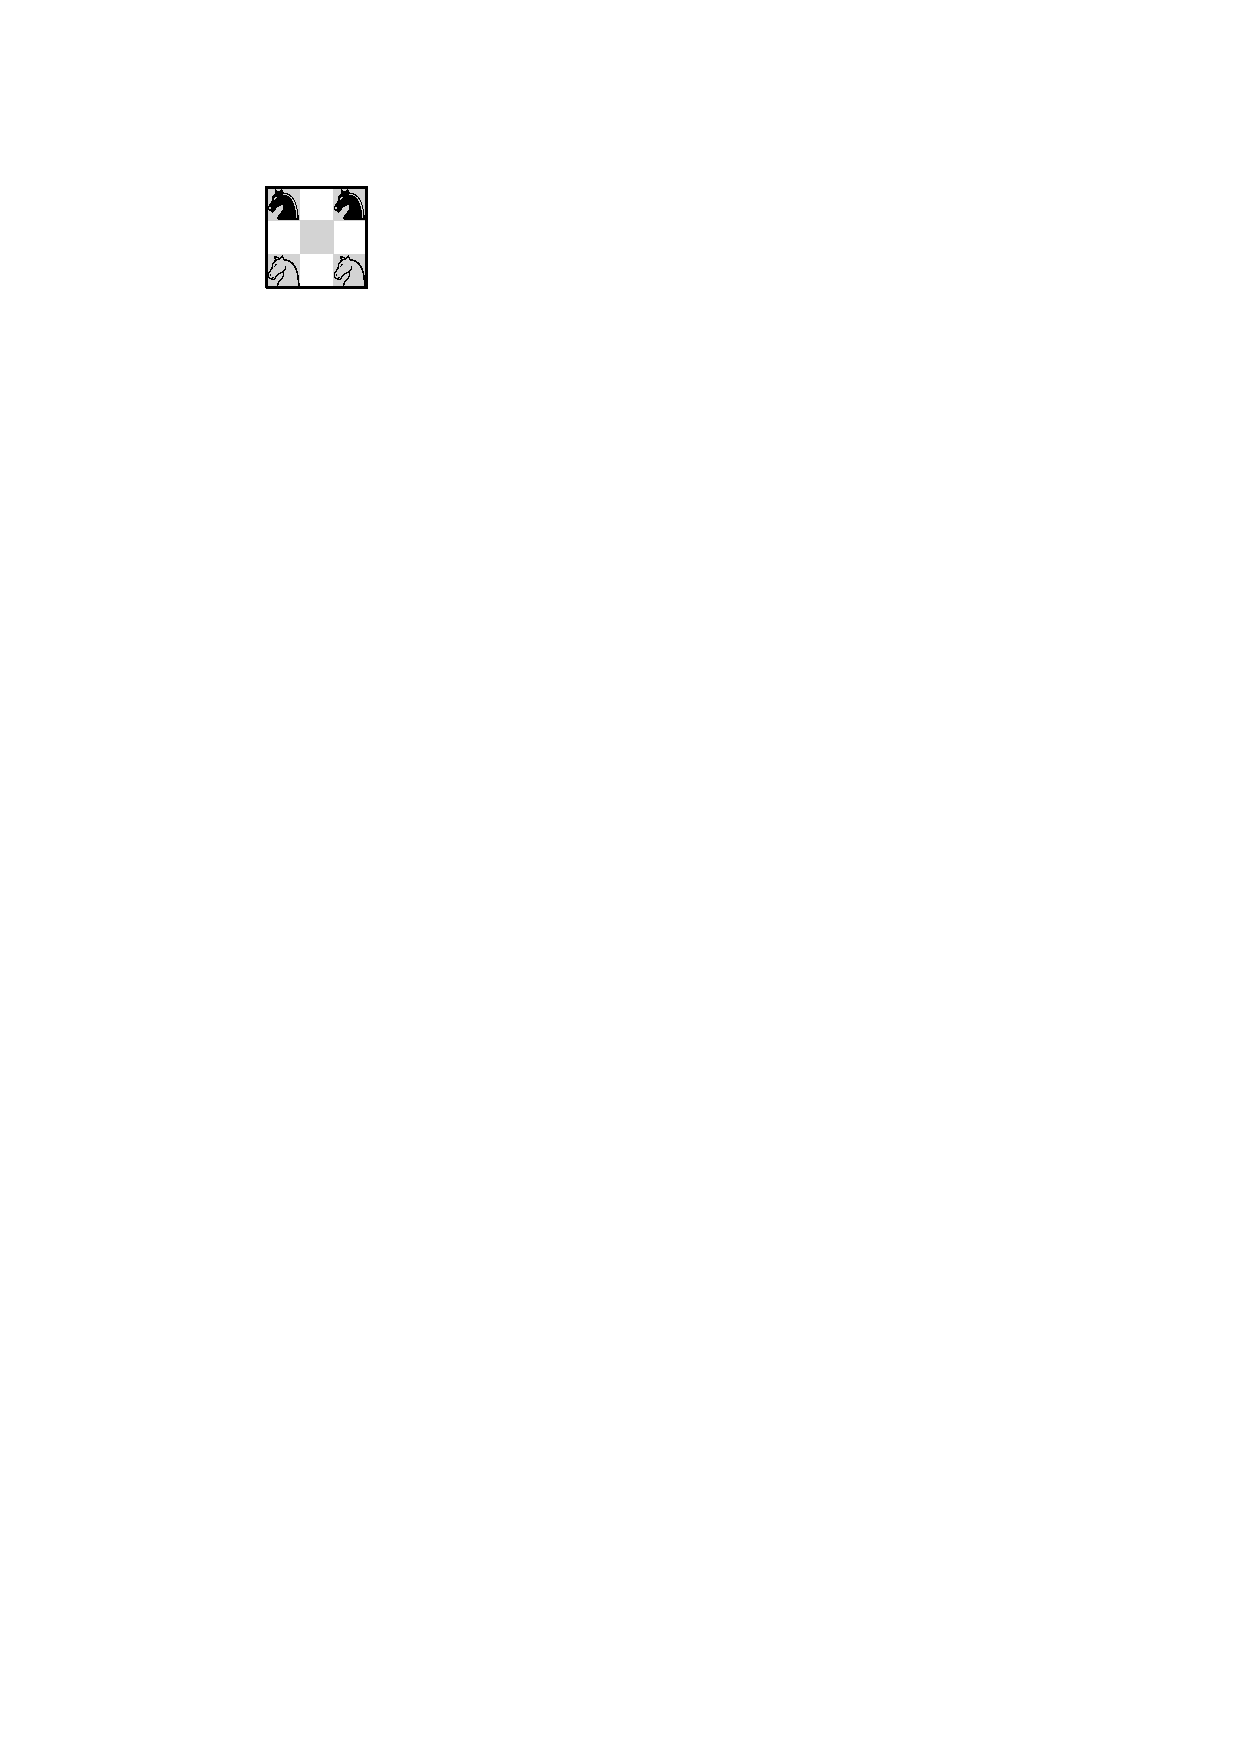
\includegraphics[scale=1.5]{img/Knights1.pdf}\qquad \qquad 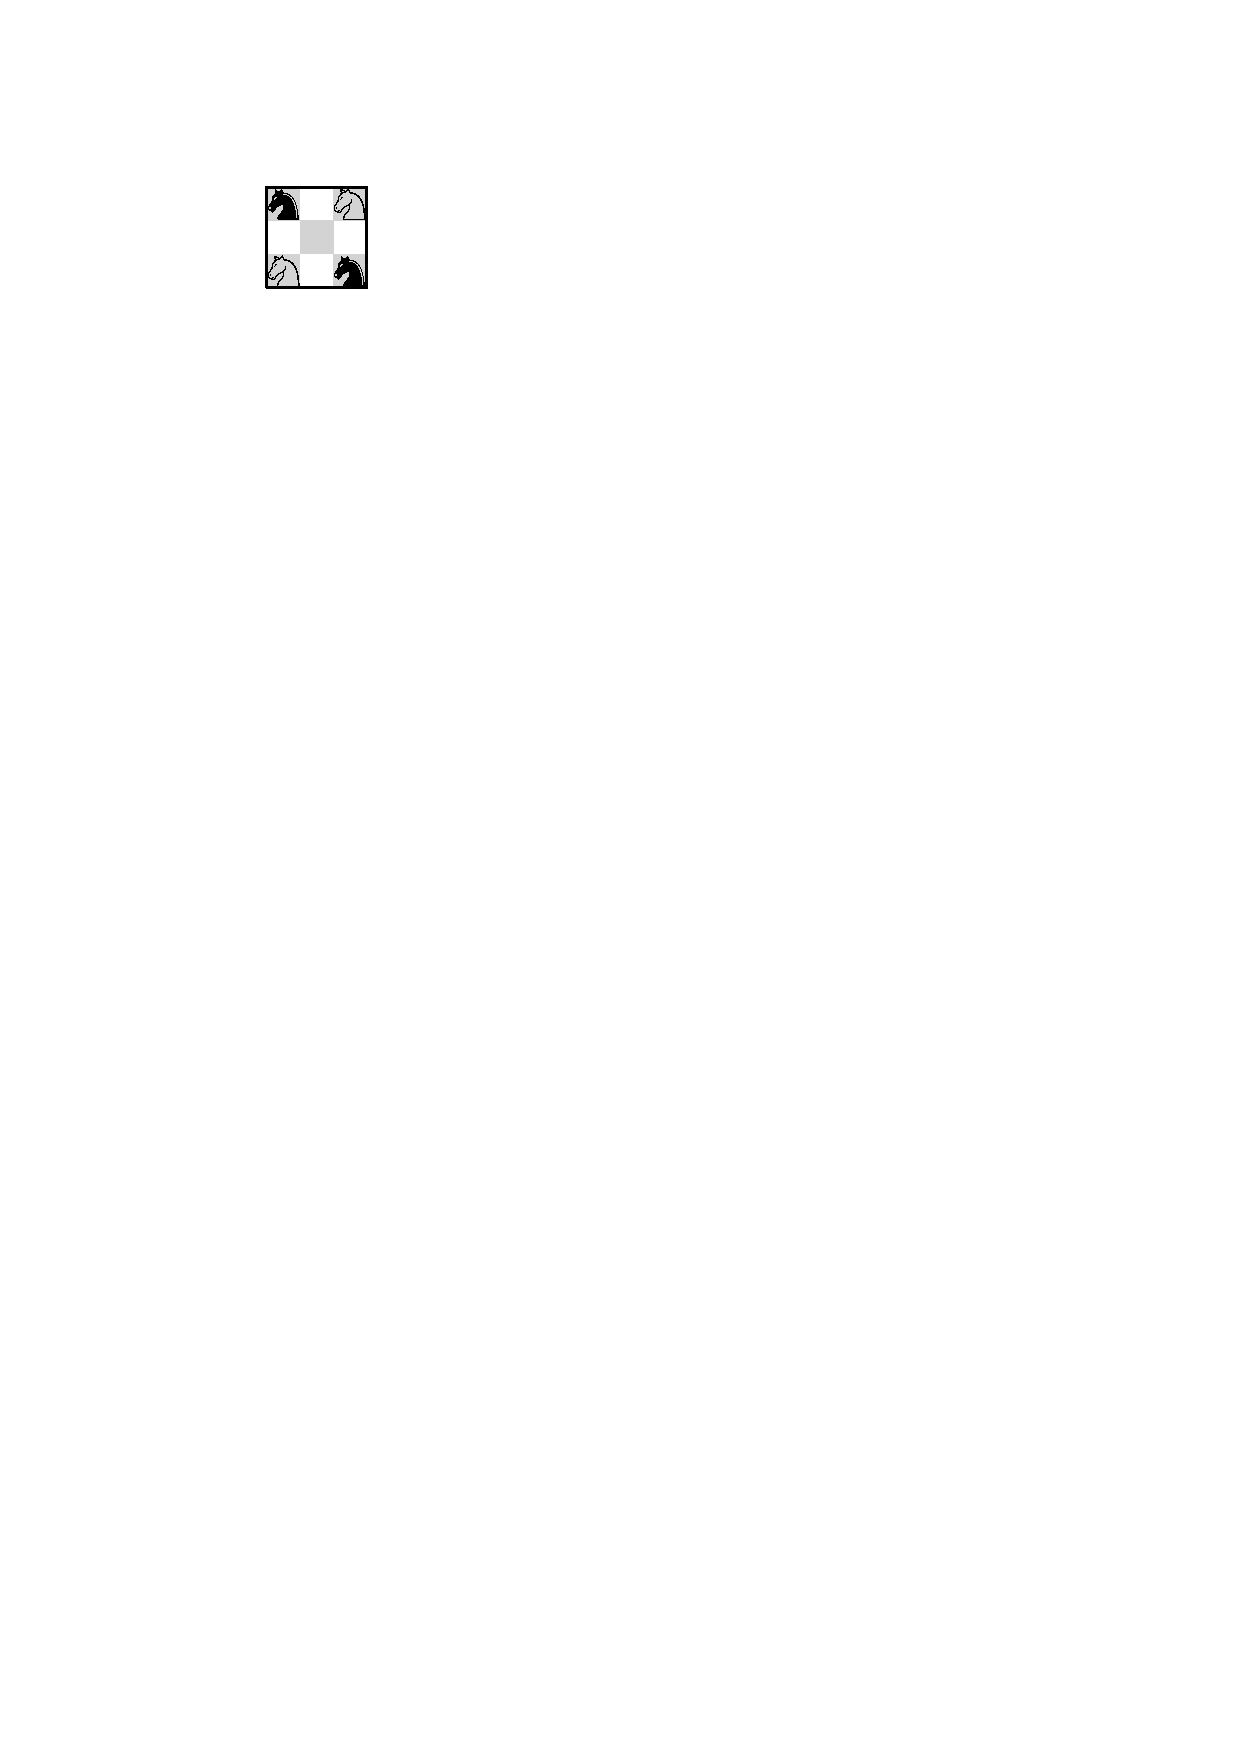
\includegraphics[scale=1.5]{img/Knights2.pdf}
\end{center}
\vspace{-25 pt}

%\z Докажите, что не существует многогранника, у которого было бы ровно семь рёбер.

%\z Докажите, что число людей, когда-либо живших на Земле и сделавших нечётное число рукопожатий, чётно.

%Бывает ли выпуклый многогранник, в котором все его 15 граней — треугольники?


\end{document}